% ------ | ------- | ------- | ------- | ------- | ------- | ------- | ------- |
%
\documentclass[twocolumn,twoside,fleqn,12pt]{article}
%
% This lightly writes DRAFT across each page.
%\usepackage{draftcopy}
%
% Handling footnotes
\usepackage{ftnright}                  % Places footnotes in right column
\setlength{\skip\footins}{8pt}         % Sets footnote size to 8pt
\addtolength{\textheight}{1in}         % Adjusts spacing for footnotes
\preparefootins                        % Saves these parameters
%
% For handling encapsulated postscript files.
\usepackage[pdftex]{graphicx}
%\usepackage{epsfig}
%
% Single column figure
%\begin{figure}
%   \centering
%   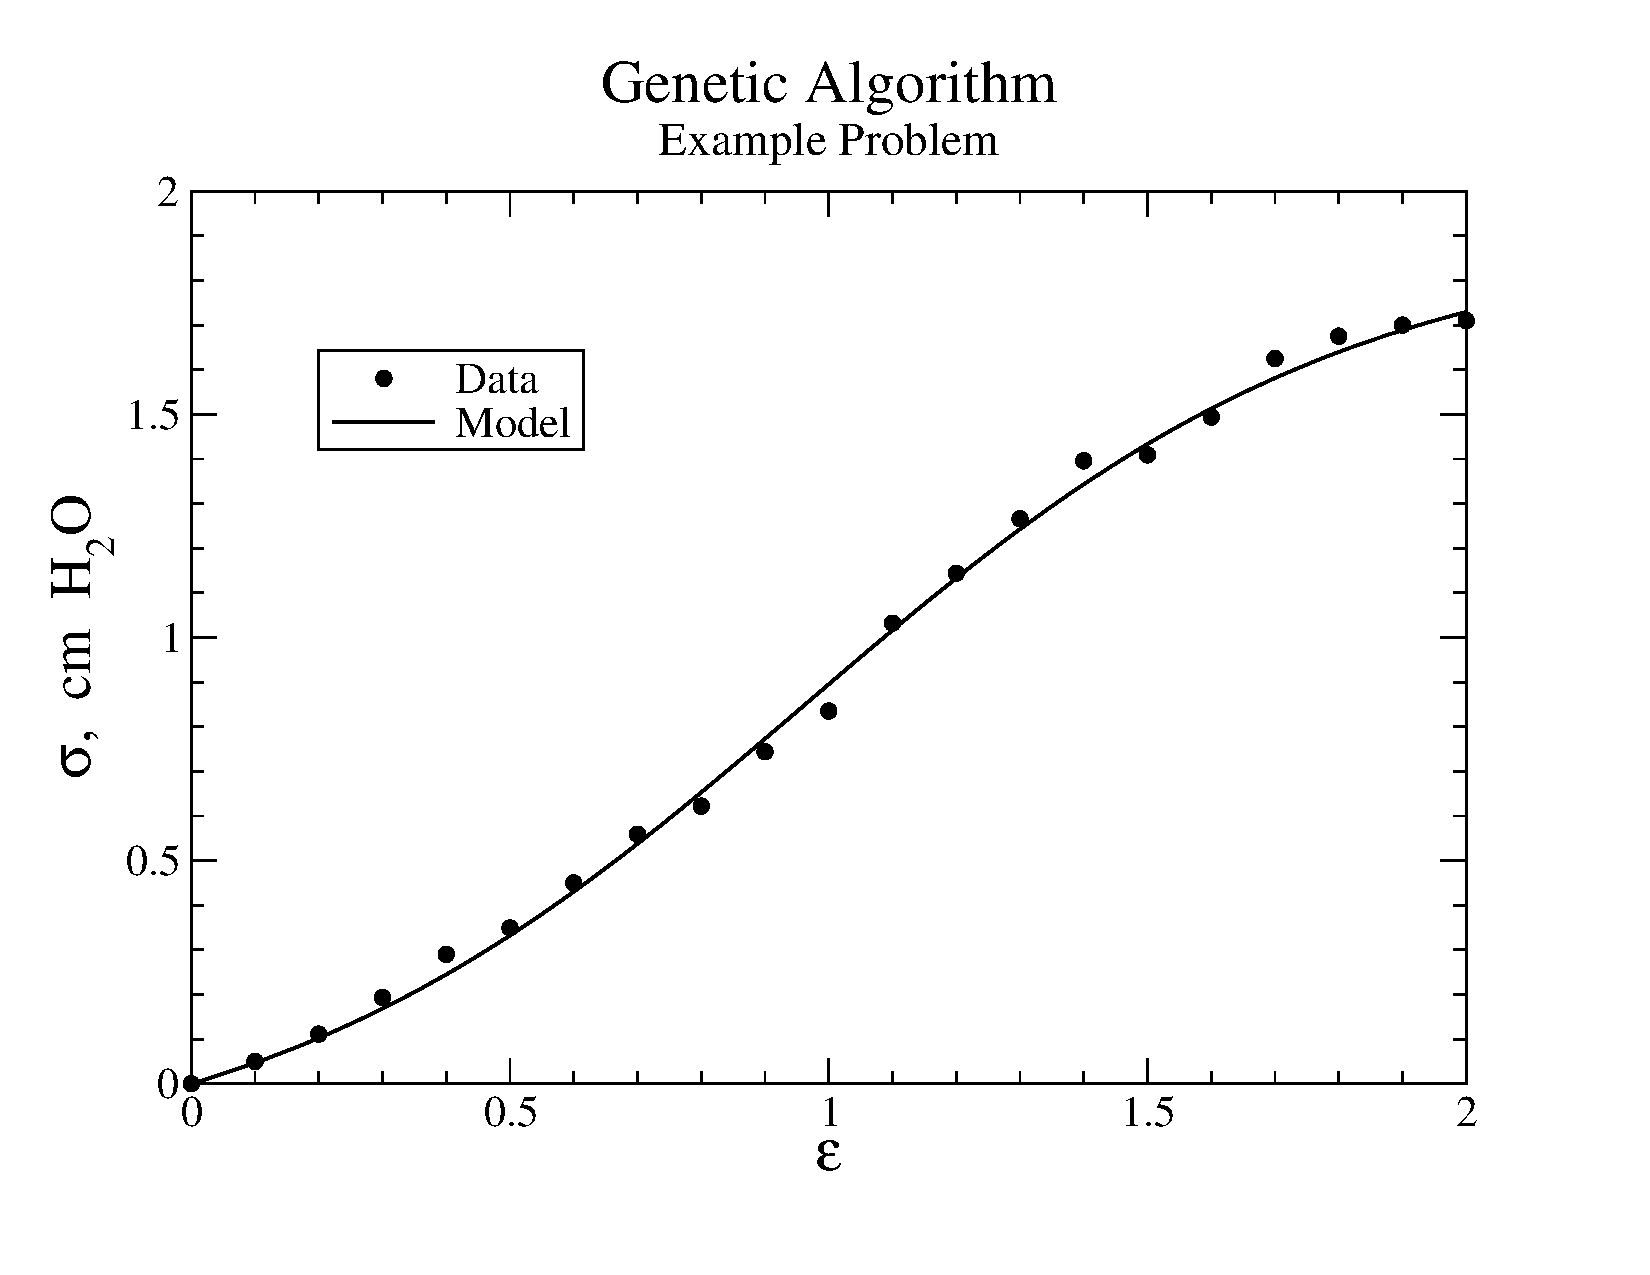
\includegraphics[angle=-90,width=8cm]{gaExample.pdf}
%   \caption{...}
%   \label{...}
%\end{figure}
%
% Double column figure
%\begin{figure*}
%   {\par\centering
%   \resizebox*{1.0\textwidth}{.25\textheight}
%   {\includegraphics[angle=-90]{<figure.eps>}}
%   \par}
%   \caption{\label{<figureLabel>}%
%   }
%\end{figure*}
%
% Tables are the same. A one column table has the structure
%\begin{table}
%  ...
%\end{table}
%
% while a two-column table is created with
%\begin{table*}
%  ...
%\end{table*}
%
%
% Set up babel for typesetting bibliographies.
\usepackage[english]{babel}  %language selection
\selectlanguage{english}
% Languages supported by babel include:
%   american, austrian, brazil, catalan, croatian, czech, danish, dutch,
%   english, esperanto, finnish, french, galician, german, italian, magyar,
%   norsk, nynorsk, polish, portuges, romanian, russian, slovak, slovene,
%   spanish, swedish, turkish.
%
% Select the default text font which is used, for example,
% in the typesetting of the front matter of a paper
% and in the typesetting text in formulae, e.g., sin.
% The Monotype Baskerville fonts are sold separately at: http://www.fonts.com.
%\renewcommand{\rmdefault}{cmr}        % computer modern roman
%\renewcommand{\rmdefault}{txr}        % TX fonts
%\renewcommand{\rmdefault}{ptm}        % Adobe times roman
%\renewcommand{\rmdefault}{mbv}        % Baskerville with inline numbers
\renewcommand{\rmdefault}{mbvj}        % Baskerville with old-style numbers
%
% If AMS-LaTeX macros are to used, load them before mtpro.
% MTPro will replace the AMS fonts, but not its macros.
\usepackage{amsmath, amsthm}
%
\usepackage{textcomp}
%
% Load MathTime Professional II fonts - commercial fonts
% For sales and other information visit www.pctex.com.
% The following math fonts are created:
%   \mathrm   \mathit    \mathsf   \mathtt
%   \mathbf   \mathbold  \mbf      \mathbb
%   \mathcal  \mathbcal  \mathscr  \mathbscr  \mathfrak
%\usepackage[subscriptcorrection,slantedGreek,boldalphabet,mtpccal,mtpscr,mtpfrak,mtphrb,zswash,nofontinfo]{mtpro2}
\usepackage[subscriptcorrection,slantedGreek,mtpccal,mtpscr,mtpfrak,mtphrb,zswash,nofontinfo]{mtpro2}
%
% Introduce the text fonts.
%
% Define a set of macros for characterizing text fonts.
%   medium fonts   roman     san serif    typewriter
%     upright     \fontrm    \fontss      \fonttt
%     slant       \fontsl    \fontsssl    \fontttsl
%     small cap   \fontsc    \fontsssc    \fontttsc
%     italic      \fontit
%
%   bold fonts     roman     san serif    typewriter
%     upright     \boldrm    \boldss      \boldtt
%     slant       \boldsl    \boldsssl    \boldttsl
%     small cap   \boldsc    \boldsssc    \boldttsc
%     italic      \boldit
%
% Establish the default font encoding scheme to use.
\DeclareFontEncoding{T1}{}{}           % specify text font encoding scheme
\DeclareFontEncoding{TS1}{}{}          % specify text companion font encoding
%
% Normal text fonts.
\DeclareFontFamily{T1}{txr}{\hyphenchar\font=127}
\DeclareFontShape{T1}{txr}{m}{n}{<-> t1xr}{}
\DeclareFontShape{T1}{txr}{m}{sl}{<-> t1xsl}{}
\DeclareFontShape{T1}{txr}{m}{sc}{<-> t1xsc}{}
\DeclareFontShape{T1}{txr}{m}{it}{<-> t1xi}{}
\renewcommand{\normalfont}{\usefont{T1}{txr}{m}{n}}
\newcommand{\fontrm}[1]{\normalfont{#1}}
\newcommand{\fontsl}[1]{\usefont{T1}{txr}{m}{sl}{#1}\normalfont}
\newcommand{\fontsc}[1]{\usefont{T1}{txr}{m}{sc}{#1}\normalfont}
\newcommand{\fontit}[1]{\usefont{T1}{txr}{m}{it}{#1}\normalfont}
%
% Bold text fonts.
\DeclareFontFamily{T1}{txb}{\hyphenchar\font=127}
\DeclareFontShape{T1}{txb}{bx}{n}{<-> t1xb}{}
\DeclareFontShape{T1}{txb}{bx}{sl}{<-> t1xbsl}{}
\DeclareFontShape{T1}{txb}{bx}{sc}{<-> t1xbsc}{}
\DeclareFontShape{T1}{txb}{bx}{it}{<-> t1xbi}{}
\newcommand{\boldrm}[1]{\usefont{T1}{txb}{bx}{n}{#1}\normalfont}
\newcommand{\boldsl}[1]{\usefont{T1}{txb}{bx}{sl}{#1}\normalfont}
\newcommand{\boldsc}[1]{\usefont{T1}{txb}{bx}{sc}{#1}\normalfont}
\newcommand{\boldit}[1]{\usefont{T1}{txb}{bx}{it}{#1}\normalfont}
%
% Normal san serif fonts.
\DeclareFontFamily{T1}{txss}{\hyphenchar\font=127}
\DeclareFontShape{T1}{txss}{m}{n}{<-> s * [0.95] t1xss}{}
\DeclareFontShape{T1}{txss}{m}{sl}{<-> s * [0.95] t1xsssl}{}
\DeclareFontShape{T1}{txss}{m}{sc}{<-> s * [0.95] t1xsssc}{}
\newcommand{\fontss}[1]{\usefont{T1}{txss}{m}{n}{#1}\normalfont}
\newcommand{\fontsssl}[1]{\usefont{T1}{txss}{m}{sl}{#1}\normalfont}
\newcommand{\fontsssc}[1]{\usefont{T1}{txss}{m}{sc}{#1}\normalfont}
%
% Bold san serif fonts.
\DeclareFontFamily{T1}{txssb}{\hyphenchar\font=127}
\DeclareFontShape{T1}{txssb}{bx}{n}{<-> s * [0.95] t1xbss}{}
\DeclareFontShape{T1}{txssb}{bx}{sl}{<-> s * [0.95] t1xbsssl}{}
\DeclareFontShape{T1}{txssb}{bx}{sc}{<-> s * [0.95] t1xbsssc}{}
\newcommand{\boldss}[1]{\usefont{T1}{txssb}{bx}{n}{#1}\normalfont}
\newcommand{\boldsssl}[1]{\usefont{T1}{txssb}{bx}{sl}{#1}\normalfont}
\newcommand{\boldsssc}[1]{\usefont{T1}{txssb}{bx}{sc}{#1}\normalfont}
%
% Normal typewriter fonts.
\DeclareFontFamily{T1}{txtt}{\hyphenchar\font=127}
\DeclareFontShape{T1}{txtt}{m}{n}{<-> t1xtt}{}
\DeclareFontShape{T1}{txtt}{m}{sl}{<-> t1xttsl}{}
\DeclareFontShape{T1}{txtt}{m}{sc}{<-> t1xttsc}{}
\newcommand{\fonttt}[1]{\usefont{T1}{txtt}{m}{n}{#1}\normalfont}
\newcommand{\fontttsl}[1]{\usefont{T1}{txtt}{m}{sl}{#1}\normalfont}
\newcommand{\fontttsc}[1]{\usefont{T1}{txtt}{m}{sc}{#1}\normalfont}
%
% Bold typewriter fonts.
\DeclareFontFamily{T1}{txttb}{\hyphenchar\font=127}
\DeclareFontShape{T1}{txttb}{bx}{n}{<-> t1xbtt}{}
\DeclareFontShape{T1}{txttb}{bx}{sl}{<-> t1xbttsl}{}
\DeclareFontShape{T1}{txttb}{bx}{sc}{<-> t1xbttsc}{}
\newcommand{\boldtt}[1]{\usefont{T1}{txttb}{bx}{n}{#1}\normalfont}
\newcommand{\boldttsl}[1]{\usefont{T1}{txttb}{bx}{sl}{#1}\normalfont}
\newcommand{\boldttsc}[1]{\usefont{T1}{txttb}{bx}{sc}{#1}\normalfont}
%
\usepackage{xspace} % provides appropriate spacing
% Redefine the standard text font selecting macros.
\renewcommand{\textrm}[1]{\fontrm{#1}\xspace}
\renewcommand{\textbf}[1]{\boldrm{#1}\xspace}
\renewcommand{\textit}[1]{\fontit{#1}\xspace}
\renewcommand{\textsc}[1]{\fontsc{#1}\xspace}
\renewcommand{\textsf}[1]{\fontss{#1}\xspace}
\renewcommand{\textsl}[1]{\fontsl{#1}\xspace}
\renewcommand{\texttt}[1]{\fonttt{#1}\xspace}
\renewcommand{\textup}[1]{\fontrm{#1}\xspace}
% If xspace provides unwanted spacing, do not use the
% base \font## or \bold## commands instead of \text##.
%
\newcommand{\eg}{e.g.,\xspace}
\newcommand{\ie}{i.e.,\xspace}
\newcommand{\viz}{viz.,\xspace}
\newcommand{\cf}{cf.\@\xspace}
\newcommand{\eq}{Eq.\@\xspace}
\newcommand{\eqs}{Eqs.\@\xspace}
\newcommand{\etc}{etc.\@\xspace}
\newcommand{\fig}{Fig.\@\xspace}
\newcommand{\figs}{Figs.\@\xspace}
\newcommand{\vs}{vs.\@\xspace}
%
% For underlining options
%\usepackage{ulem}
%    \uline{important}   underlined text
%    \uuline{urgent}     double-underlined text
%    \uwave{boat}        wavy underline
%    \sout{wrong}        line drawn through word
%    \xout{removed}      marked over with //////
%
% Define macros for writing tensor equations.
%
% Macro for typesetting numbers in text.
\newcommand{\scalar}[1]%
   {\fontencoding{TS1}\selectfont #1\fontencoding{T1}\selectfont}
%
% Macros for typesetting vectors - italic roman.
\DeclareMathAlphabet{\mathitbb}{U}{mt2hrb}{m}{it}
\newcommand{\vecFld}[1]{\ensuremath{\mathbold{#1}}}
\newcommand{\vecEle}[1]{\ensuremath{\mathit{#1}}}
\newcommand{\vecMtx}[1]{\ensuremath{\mathitbb{#1}}}
%
% Macros for typesetting tensors of second rank - upright roman.
\newcommand{\tenFld}[1]{\ensuremath{\mbf{#1}}}
\newcommand{\tenEle}[1]{\ensuremath{\mathrm{#1}}}
\newcommand{\tenMtx}[1]{\ensuremath{\mathbb{#1}}}
%
% Macros for typesetting tensors of fourth rank - italic san serif.
\DeclareMathAlphabet{\mathsfbb}{U}{mt2bb}{m}{it}
\newcommand{\TenFld}[1]{\ensuremath{\text{\boldsssl{#1}}}}
\newcommand{\TenEle}[1]{\ensuremath{\text{\fontsssl{#1}}}}
\newcommand{\TenMtx}[1]{\ensuremath{\mathsfbb{#1}}}
%
% Macros for typesetting greek symboled fields.
\newcommand{\grkFld}[1]{\ensuremath{\mathbold{#1}}}
\newcommand{\grkEle}[1]{\ensuremath{#1}}
\newcommand{\grkMtx}[1]{\ensuremath{\mathitbb{#1}}}
%
% Macros for creating nice text and script fractions.
%   There is a cleaner way to do this; for example,
%   \newcommand*{\textfrac}[2]{%
%      {\fontfamily{<fontname>1}\selectfont #1}%
%      \textfractionsolidus
%      {\fontfamily{<fontname>0}\selectfont #2}}%
%   See http://www.ctan.org/tex-archive/macros/latex/doc/fntguide.pdf
%   Sec. V.5: Using the feature of expert fonts
%   Here we must use the following hack because Adobe Times Roman and
%   Baskerville expert fonts do not contain the superior <fontname>1
%   and inferior <fontname>0 glyphs in their font tables.
% Do not break these long lines into multiple lines
% Spaces CANNOT be present - they cause unwanted `rubber' spacing
\newcommand{\textfrac}[2]
   {\leavevmode
    \kern.05em\raise.6ex\hbox{\ensuremath{\scriptstyle{#1}}}\kern-.05em\hspace{0em}/\hspace{0em}\kern-.05em\lower.2ex\hbox{\ensuremath{\scriptstyle{#2}}}\kern.05em
   }
\newcommand{\scriptfrac}[2]
   {\leavevmode
    \kern.05em\raise.3ex\hbox{\ensuremath{\scriptscriptstyle{#1}}}\kern-.05em\hspace{0em}\hbox{\ensuremath{\scriptstyle{/}}}\hspace{0em}\kern-.05em\lower.25ex\hbox{\ensuremath{\scriptscriptstyle{#2}}}\kern.05em
   }
%
% Layout and formatting of the document.
%
% page size
\pdfpagewidth 8.5in
\pdfpageheight 11in
% top margin
\setlength\topmargin{-0.25in}
% header properties
\setlength\headheight{0in}
\setlength\headsep{0in}
% printed size on paper
\setlength\textheight{9.5in}
\setlength\textwidth{7in}
% margins for two-sided printing
\setlength\oddsidemargin{0in}
\setlength\evensidemargin{-0.4in}
% paragraph properties
\setlength\parindent{0.25in}
\setlength\parskip{0.05in}
% Column separation
\setlength{\columnsep}{15pt}
\setlength{\columnseprule}{0pt}
% Fill page
\flushbottom
%
%
% don't hyphenate so much - default = 200, max (never hyphenate) = 10,000
\hyphenpenalty=800
%
% two column float page must be 90% full
\renewcommand\dblfloatpagefraction{.90}
% two column top float can cover up to 80% of page
\renewcommand\dbltopfraction{.80}
% float page must be 90% full
\renewcommand\floatpagefraction{.90}
% top float can cover up to 80% of page
\renewcommand\topfraction{.80}
% bottom float can cover up to 80% of page
\renewcommand\bottomfraction{.80}
% at least 10% of a normal page must contain text
\renewcommand\textfraction{.1}
%
% separation between floats and text
\setlength\dbltextfloatsep{9pt plus 5pt minus 3pt }
% separation between two column floats and text
\setlength\textfloatsep{10pt plus 4pt minus 3pt}
%
%
% Macro used for creating nomenclatures, etc.
\newcommand{\namelistlabel}[1]{\mbox{#1}\hfil}
\newenvironment{namelist}[1]
   {\begin{list}{}%
      {\let\makelabel\namelistlabel%
       \settowidth{\labelwidth}{#1\hphantom{ }}%
       \setlength{\leftmargin}{\labelwidth}%
       \setlength{\itemsep}{-6pt}%
      }%
   }{\end{list}%
}
%
% Additional declarations beyond my standard template.
%
%%%%%%%%%%%%%%%%%%%%%%%%%%%%%%%%%%%%%%%%%%%%%%%%%%
%
%
%
\begin{document}
%
\bibliographystyle{asme}       % numeric bibliography format
%\bibliographystyle{plain}
%
\title{Zonnon\\
       A Quick Reference Guide\\
       \phantom{A}}
%
\author{Alan D.\ Freed\\
\and
\mbox{}\hfill Clifford H.\ Spicer Chair in Engineering\\
\mbox{}\hfill College of Science, Engineering \& Technology\\
\mbox{}\hfill Saginaw Valley State University\\
\mbox{}\hfill 202 Pioneer Hall, 7400 Bay Road\\
\mbox{}\hfill University Center, MI 48710\\
\mbox{}\hfill E-Mail: \texttt{adfreed@svsu.edu}\\
}
%
\date{draft copy \\ \today}

\maketitle
\normalfont

\begin{abstract}
   Write abstract
\end{abstract}

\section{Introduction}

\textsf{Zonnon} is the most recent language in the 
\textsf{Euler}\slash\textsf{Algol}\slash\textsf{Pascal}\slash
\textsf{Modula}\slash\textsf{Oberon} family of programming languages
developed by Profs.\ Niklaus Wirth and J\"urg Gutknecht from the Computer
Systems Institute at ETH Zurich (Eidgen\"ossische Technische Hochschule,
Z\"urich, \ie the Swiss Federal Institute of Technology, Zurich). 
Eugene Zueff, Roman Mitin and Nina Gonova, students and research 
affiliates at ETH Zurich, were the primary compiler developers.
The \textsf{Zonnon} compiler, limited documentation, and example 
programs are available for download from their website
\texttt{http:\slash\slash www.zonnon.ethz.ch}.

To date, no textbook has been written in English that describes 
how to program in \textsf{Zonnon}.  A tutorial, originally written 
in Russian, has been translated into English by its author, 
Roman Mitin, but, like this document,
it is not in a finished state at this time.
This document is not a substitute for a textbook on \textsf{Zonnon},
but it might be useful as a quick reference guide to refer to when
a programming question arises to those learning the language.
This guide does not cover all of the capabilities of the language,
as its intent is for the novice to use as a resouce next to them
when they are writing code on the computer.

\section{Comments}

It is good parctice to begin each program file with a few comment
statements that identify who you are, the programmer, what the date is,
and any necessary affiliations.  This header should also contain a brief
statement as to what this particular code is suppose to do, or
why it was written, if it is copyrighted, or under a license of some
kind or another, \eg
\begin{verbatim}
(* Joe Student, XYZ University *)
(* today's date                *)
(* Programming Assignment #1   *)
\end{verbatim}
A comment statement in \textsf{Zonnon} begins with \texttt{(*} and
ends with \texttt{*)}, as seen above.  It is not necessary to place
each line in a comment.  Comments may span over how
many ever lines of code you choose, and may begin at any position
within a line of code.  They may even be nested, but each opening
\texttt{(*} must be paired with a closing \texttt{*)}.

\section{Words}

There are two kinds of words that the programmer has at their disposal.
The first set includes the \textit{reserved words\/} of the language,
while the second set includes the words the programmer creates to
describe an entity to be represented.  An alphabetical listing of the
reserved words that make up the \textsf{Zonnon} language includes:
\boldrm{accept}, \boldrm{activity}, \boldrm{array}, \boldrm{as},
\boldrm{await}, \boldrm{begin}, \boldrm{by}, \boldrm{case}, \boldrm{const},
\boldrm{definition}, \boldrm{div}, \boldrm{do}, \boldrm{else},
\boldrm{elsif}, \boldrm{end}, \boldrm{exception}, \boldrm{exit},
\boldrm{false}, \boldrm{for}, \boldrm{if}, \boldrm{implementation},
\boldrm{implements}, \boldrm{import}, \boldrm{in}, \boldrm{is},
\boldrm{loop}, \boldrm{mod}, \boldrm{module},
\boldrm{new}, \boldrm{nil}, \boldrm{object}, \boldrm{of}, \boldrm{on},
\boldrm{operator}, \boldrm{or}, \boldrm{procedure}, \boldrm{protocol},
\boldrm{record}, \boldrm{refines}, \boldrm{return}, \boldrm{self},
\boldrm{termination}, \boldrm{then}, \boldrm{to}, \boldrm{true},
\boldrm{type}, \boldrm{until}, \textbf{var} and \boldrm{while}.
As the compiler currently stands, these reserved
words must be used in lower case. Although the language definition
permits them to be used either in all lower-case or in all upper-case,
that feature has not been implemented yet.

An admissible word that the programmer can create contains an ensemble
of any English letter ``a''|$\dots$|``z''|``A''|$\dots$|``Z'', the
underscore ``_'', and any digit ``0''|$\dots$|``9''.  It can be of
arbitrary length, but it cannot begin with a digit.  Good word choice
goes a very long way to readability of a code.  Mixing the case allows
the programmer to use an otherwise reserved word, \eg \texttt{Object}
could be used by the programmer as a programmer defined entity.  In
the code fragments throughout this guide, user defined words are
expressed in angled brackets like \texttt{<userWord>}.

A \textit{program\/} is a collection of words arranged in such a manner
that, collectively, they become understandable to the \textsf{Zonnon}
compiler.  A program is a text file ending in a `.znn' extension.  It can
be written in any text editor of your choice.  Several have highlighting
features that recognize the reserved words, thereby aiding in the overall
coding process, \eg Kate or the editor in Zonnon Builder that comes
with the Windows$^{\text{TM}}$ version of the compiler.

\section{Basic Types}

There are a number of base types in the \textsf{Zonnon} language that
provide a foundation upon which the programmer can build applications,
and even other types of user specification.  These core types are:
\begin{namelist}{cardinal}
   \item[\textbf{boolean}] A truth value of either \textbf{true} or
      \textbf{false}.
   \item[\textbf{cardinal}] A counting number beginning at 0 and going to
      \textbf{max(cardinal)}.
   \item[\textbf{char}] Any character from the character set of your
      system, \eg ASCII or UTF8.
   \item[\textbf{integer}] A counting number between \textbf{min(integer)}
      and \textbf{max(integer)}, where |\boldrm{min(integer)}| = 1 +
      \textbf{max(integer)}.
   \item[\textbf{object}] The base type from which all user-defined
      \textsf{Zonnon} objects are derived.
   \item[\textbf{real}] A floating point number with values between
      \textbf{min(real)} and \textbf{max(real)}.
   \item[\textbf{string}] A concatenation of characters from the base
      character set.
\end{namelist}
Types \boldrm{cardinal}, \boldrm{char}, \boldrm{integer} and \textbf{real}
can be used in different sizes by specifying their length in bits
inside a pair of braces \{ and \} immediately following the type name,
\eg \boldrm{real}\{32\} associates with a 32-bit real.  The default
sizes are: \boldrm{cardinal}\{32\}, \boldrm{char}\{16\},
\boldrm{integer}\{32\} and \boldrm{real}\{64\}.  Type \textbf{char}
also comes in an 8-bit size; types \textbf{cardinal} and \textbf{integer}
also come in 8-, 16- and 64-bit sizes; and type \textbf{real} also
comes in a 32-bit size.

\textsf{Zonnon} base types that are not listed above include: \boldrm{fixed},
\textbf{range} and \textbf{set}, as they are not discussed in this document.

\subsection{Operators}

Instances of types can be combined to create new instances through a
variety of operators.  Instances of type \textbf{string} can be
concatenated with the \texttt{+} operator.  The numeric types of
\boldrm{cardinal}, \textbf{integer} and \textbf{real} have a unary
operator \texttt{-} used for negation (except \textbf{cardinal}
numbers which do not admit negative numbers), and binary operators
for addition \texttt{+}, subtraction \texttt{-}, multiplication
\texttt{*} and exponentiation \texttt{**}.
\textbf{real} division has the operator \texttt{/}, while
\textbf{cardinal} and \textbf{integer} division have operators
\texttt{div} and \texttt{mod} returning the divisor and remainder,
respectively.  Binary operators for comparing two numeric values are
equal \texttt{=}, not equal \texttt{\#}, less than \texttt{<},
less than or equal \texttt{<=}, greater than \texttt{>}
or greater then or equal \texttt{>=}, each returning a
\textbf{boolean} result.

For \textbf{boolean} instances, there are three operators: the uniary
operator \textasciitilde\ for negation, and the binary operators \texttt{\&}
for logical and, and \texttt{or} for logical or.  Two \textbf{boolean}
instances can also be compared with operators \texttt{=} and \texttt{\#}.

When a line of code is parsed by the compiler, execution is left to right
unless terms are grouped with parentheses \texttt{(} and \texttt{)}.
Operator precedence from highest to lowest is:
\begin{enumerate}
 \item unary operations \texttt{-} and \textasciitilde
 \item exponentiation operator \texttt{**}
 \item multiplication operators \texttt{*}, \texttt{/}, \texttt{div}
   and \texttt{mod}
 \item addition operators \texttt{+} and \texttt{-}
 \item relations \texttt{=}, \texttt{\#}, \texttt{<}, \texttt{<=},
   \texttt{>} and \texttt{>=}
\end{enumerate}

\section{Statements}

Statements are used for two purposes: assignment and comparison.  An
\textit{assignment statement\/} has three parts to it, as shown below.
\begin{verbatim}
<receiver> := <sender>;
\end{verbatim}
A statement may span several lines of code.  It ends with a semicolon.
In the statement above, entity \texttt{<sender>} on the right-hand
side is \textit{assigned\/} by the operator \texttt{:=} to entity
\texttt{<receiver>} on the left-hand side.  \textsf{Zonnon} is a
strongly typed language.  This means that the type which instance
\texttt{<receiver>} belongs to must be compatible with the type which
instance \texttt{<sender>} belongs to.  The compiler will produce an error
message if their declared types are not compatible with one another.

Within a scope, a sequence of statements might look like:
\begin{verbatim}
begin
   <receiver1> := <sender1>;
   <receiver2> := <sender2>;
   ...
   <receiverN> := <senderN>
end;
\end{verbatim}
Notice that the last assignment statement in a scope does not need to
close with a semicolon.  It can, it just doesn't have to.

A \textit{comparison statement\/} also has three parts to it, as shown below.
\begin{verbatim}
<left> =  <right>;
<left> #  <right>;
<left> <  <right>;
<left> <= <right>;
<left> >  <right>;
<left> >= <right>;
\end{verbatim}
These statements compare the value held by \texttt{<right>} with the value
held by \texttt{<left>}, and report on the outcome of the associated truth
test.  A comparison statement takes
on the result of its associated truth test, \ie it can be either
\textbf{true} or \textbf{false}.  Once again, the strong typing of
\textsf{Zonnon} requires that the type belonging to instance \texttt{<right>}
must be compatible with the type belonging to instance \texttt{<left>},
and such operators must be defined for said type, otherwise the compiler
will output an error message.

\section{Declarations}

Two different types of declaration blocks are provided for: constants
and variables.  A \textit{constant declaration\/} associates an
identifier with its value.
\begin{verbatim}
const
   <name1> = <value1>;
   <name2> = <value2>;
\end{verbatim}
Two things are worthy of notice here.  The list of constants are semicolon
separated, and the equality operator \texttt{=}, not the assignment
operator \texttt{:=}, associates the identifier with its value.

A \textit{variable declaration\/} has the following structure.
\begin{verbatim}
var {private|public|public, immutable}
   <name1T1>, ..., <nameNT1> : <type1>;
   <name1T2>, ..., <nameNT2> : <type2>;
   ...
   <name1TM>, ..., <nameNTM> : <typeM>;
\end{verbatim}
The instances of a type are placed to the left of the colon, while the type
that they associate with is to the right of the colon.  Instances are comma
separated, while type clauses are semicolon separated.  All variables
declared in a \textbf{var} block are either \texttt{private} (visible
only inside the scope of their definition), or \texttt{public} (visible
and writable outside the scope of their definition), or \texttt{public},
\texttt{immutable} (read-only outside the scope of their definition).
Multiple \textbf{var} blocks are permitted so that all necessary
instances of each visibility case can be dealt with.

\section{Types}

Two kinds of user-defined types are now discussed; they are the
\textbf{array} and \textbf{enumeration} types.  Later, the
\textbf{procedure}, \textbf{record} and \textbf{object} types will
also be discussed.  Not addressed in this introductory guide are
the \textbf{activity}, \textbf{interface} and \textbf{protocol}
types, which are very powerful, but whose use lies beyond the
capabilities of an introductory course.

\subsection{Arrays}

An \textbf{array} is a collection of elements that are instances of the
same type. They can either be created as \texttt{value} (\ie static) or
\texttt{ref} (\ie dynamic, by pointer) entities, \eg
\begin{verbatim}
type {private|public}
   <staticArrayType>
      = array <length> of <dataType>;
   <dynamicArrayType>
      = array * of <dataType>;
\end{verbatim}
where \texttt{<length>} is any cardinal value, while \texttt{*}
acts as a wild card, implying that the size of the array will be
established by the user at runtime.  Declaring these arrays takes
on the form
\begin{verbatim}
var
   <staticArray>  : <staticArrayType>;
   <dynamicArray> : <dynamicArrayType>;
begin
   <dynamicArray>
      := new <dynamicArrayType>(<rows>);
\end{verbatim}
so a \texttt{<staticArray>} only requires its \textbf{var}
declaration by the programmer, while a \texttt{<dynamicArray>}
also needs to be allocated with a call to \textbf{new}.  The advantage
here is that the number of \texttt{<rows>} that are to be assigned
to \texttt{<dynamicArray>} need not be known a~priori, only at runtime.

Arrays can be of multiple dimensions, and are created by replacing
\texttt{<length>} with \texttt{<length1>}, \texttt{<length2>}, ...,
\texttt{<lengthN>} in a static allocation, or by replacing \texttt{*}
with \texttt{*}, \texttt{*}, ..., \texttt{*} for a dynamically
allocated array.  There needs to be one designator, either
\texttt{<length>} or \texttt{*}, for each dimension desired.

The length of an array can be retrieved by calling the reserved word
\textbf{len} in one of two ways, either as \texttt{<length> :=
len(<array>)} for a one-dimensional array, or as \texttt{<rows> :=
len(<matrix>,0)} or as \texttt{<columns> := len(<matrix>,1)}
for, in this case, a two-dimensional array, \etc

Elements of an array can be either assigned to or retrieved from an indexer,
which takes the form of `\texttt{<array>[<index>]}' for a one-dimensional
array, `\texttt{<matrix>[<index>,<index>]}' for a two-dimensional array
or matrix, \etc  Admissible values for an \texttt{<index>}
range from \texttt{0} to \texttt{len(<array>) - 1}, and similarly for
multi-dimensioned arrays. An example of assigning and retrieving values is
\begin{verbatim}
<matrix>[<row>,<column>] := <setValue>;
<getValue> := <matrix>[<row>,<column>];
\end{verbatim}

There is a \texttt{\{math\}} modifier for arrays that is not discussed
here.  This feature turns on a number of performance enhancements, and
an extra syntax for arrays, making their handling more mathematical like.
The interested reader is refered to to \textsf{Zonnon} Language
Report.\footnote{The \textsf{Zonnon} Language Report is available from
the \textsf{Zonnon} website: \texttt{http:\slash\slash www.zonnon.ethz.ch}.}

\subsection{Enumeration}

An enumerated type is one that can assume only a select and known number
of values, \eg the suits in a deck of cards, or the pieces in the game of
chess, \etc  Use of these types enhances the readability of code, which
is the main strength in its usage.  They are created as
\begin{verbatim}
type {private|public}
   <enumeratedType>
      = (<value1>, ..., <valueN>);
\end{verbatim}
When used in coding, an instance of an enumerated type would be identified
as, \eg \texttt{<enumeratedType>.<valueN>}.

\section{Control Structures}

Contol structures in a computer language are used to direct the flow
of an algorithm.  Two such structures are discussed below: the
\textbf{if} and \textbf{case} statements.

\subsection{If Statement}

The \textbf{if} statement can take on one of three forms.  The first control
structure executes an extra section of code whenever a comparison statement
returns a \textbf{true}, as shown below.
\begin{verbatim}
if <truthTestIsTrue> then
   <statements>
end;
\end{verbatim}
In the second control structure, there are different sequences of statements
to be executed for both outcomes of a comparison statement.
\begin{verbatim}
if <truthTestIsTrue> then
   <statementsWhenTrue>
else
   <statementsWhenFalse>
end;
\end{verbatim}
And the third control structure applies whenever there are multiple
comparison statements to test against, in which case it looks like
the following.
\begin{verbatim}
if <truthTest1IsTrue> then
   <statements1>
elsif <truthTest2IsTrue> then
   <statements2>
...
elsif <truthTestNIsTrue> then
   <statementsN>
else
   <statementsWhenAllAreFalse>
end;
\end{verbatim}
There is no restriction on the number of \textbf{elsif} repeat clauses
that one uses.  Control ratchets down the structure until a truth test
returns \textbf{true}, or the \textbf{else} clause is reached.  After
executing the ensuing statements, programmatic flow continues with the
line of code immediately following the \textbf{if} structure.

It is good programming practice to always use an \textbf{else} segment
whenever an \textbf{elsif} clause is present so that the structure can
handle the all-false scenario.  If an all-false
scenario is encountered during a runtime, and no \textbf{else} leg
is available for escape from the logic structure of the
if-then-else statement, than a runtime error will be thrown.

\subsection{Case Statement}

A \textbf{case} statement is similar to an \textbf{if} statement in
its function.  The syntax is quite different though.  These control
structures work well with instances of an enumeration type, and look like
\begin{verbatim}
var
   <item> : <enumerationType>;
begin
   case <item> of
      <item>.<value1> :
         <statements1>
   |  <item>.<value2> :
         <statements2>
   |  <item>.<value3> :
         <statements3>
   ...
   else
      <statements>
   end;
\end{verbatim}
A colon is used to separate the testing of the condition from the code
that is to be executed after a favorable test.  Like in an \textbf{if}
statement, if a condition of test is not favorable, the control of
programmatic flow moves to the next block in the \textbf{case} structure.
These blocks are separated by the delimiter of |, which is the analog of
an \textbf{elsif} in the if-then-else structure, with
the final block being designated with an \textbf{else} identifier, as
in an \textbf{if} structure.

This control structure also works with expressions that are instances
of type \textbf{char}, \ie the \texttt{<item>} in the above example is
a character, where the \texttt{<item>.<value>} is a character, \eg ``C'',
or a range of characters, \eg ``A''..``F''.

\section{Looping Structures}

There are four types of looping structures available for the programmer
to use in the \textsf{Zonnon} language: the \textbf{for} loop, the
\textbf{while} loop, the \textbf{repeat} loop, and a generic \textbf{loop}
structure.  These structures execute a sequence of statements contained
within them a multiple number of times, terminating their sequential
processing in a manner dictated by the kind of looping structure that
is in control.  Looping structures can be nested.

\subsection{For Loops}

This looping structure is often used when managing arrays.  Here an
indexer is systematically incremented from one looping iteration to
the next, terminating when the incrementor reaches or surpasses an
assigned limit.  A \textbf{for} loop has the structure
\begin{verbatim}
for <integerAssignmentStatement>
   to <limit> by <increment> do
      <statements>
end;
\end{verbatim}
where an example of \texttt{<integerAssignmentStatement>} might
look like \texttt{i := 1}.  The \textbf{to} clause states what the
upper \texttt{<limit>} of incrementing \texttt{i} would be, while
the \textbf{by} clause specifies how much each increment is to
advance by.  When not present, the \textbf{by} clause is taken to
be \texttt{1} by default.

For example, \texttt{for i := 10 to 0 by -2 do}
would set the value for \texttt{i} to \texttt{10} in the first pass
through \texttt{<statements>}, \texttt{8} in the second pass, \etc,
and exiting out of the \textbf{for} structure after completing the
pass where the value of \texttt{i} is at \texttt{0}.

\subsection{While Loops}

In a \textbf{while} loop, the test for looping occurs at the beginning
of the structure, and it is possible that it will fail on its intial
test, thereby forgoing the structure altogether.  If the test condition
has the value \textbf{true}, then enterance into the structure is permitted.
Programmatic control moves onto the next line of code after exiting the
\textbf{while} loop, which happens whenever the test condition turns up
\textbf{false}.
\begin{verbatim}
while <logicalTestIsTrue> then
   <statements>
end;
\end{verbatim}

\subsection{Repeat Loops}

A \textbf{repeat} loop is the anthesis of the \textbf{while} loop.  A
\textbf{repeat} loop is executed at least once.  Here the test condition
for exiting the loop occurs at the end of the structure.  The code within
the \textbf{repeat} block is repeated if the test condition returns
\textbf{false}, with programmatic control moving beyond the looping
structure only when the test condition returns \textbf{true}.
\begin{verbatim}
repeat
   <statements>
until <logicalTestIsTrue>;
\end{verbatim}

\subsection{A Generic Loop}

A common need when writing code is the ability to handle multiple exit
strategies in a looping algorithm.  This can be dealt with by using
the generic \textbf{loop} structure.  Actually, all of the previous
looping structures are special cases of this structure, which takes
the form
\begin{verbatim}
loop
   <statements>;
   if <logicalTest1IsTrue> then exit end;
   <statements>;
   if <logicalTest2IsTrue> then exit end;
   ...
   if <logicalTestNIsTrue> then exit end;
   <statements>
end;
\end{verbatim}
Programmatic control leaves the scope of its \textbf{loop} structure
whenever an \textbf{exit} statement is executed.

\section{Procedures}

There are three types of procedures in programming, and all use the
syntax of \textbf{procedure} in the \textsf{Zonnon} language: the command,
the function, and the procedure.

A command has the simplest form.  Commands are used whenever an action
is to be taken, and look like
\begin{verbatim}
procedure {private|public} <name>;
var
   <variableDeclarations>;
begin
   <statements>
end <name>;
\end{verbatim}
An example would be something like \texttt{Log.Close} to close a log file.

A function returns an instance of a type, and usually has an argument
being supplied to it, sometimes several.  It has a general structure of
\begin{verbatim}
procedure {private|public} <name>
   (<values> : <valType) : <returnType>;
var
   <returnValue> : <returnType>;
begin
   <statements>;
   return <returnValue>
end <name>;
\end{verbatim}
The function call \texttt{y := sin(x)} would be an example.  There can
be multiple arguments of multiple types.  If there is more than one
agrument of a given type, then that list is comma separated.  Lists
between multiple types are semicolon separated.  Like in a \textbf{var}
declaration, a list of instances belonging to a type are separated from
the type they are being designated to by a colon.  After the argument
list closes with a parenthesis \texttt{)}, a colon appears followed
by the type name belonging to the value being returned.

The final kind of procedure is a \textbf{procedure}.  Here arguments
can be of two kinds: those passed by value (as in the previous example)
and those passed by reference, \ie that follows a \textbf{var} in
the argument list.
\begin{verbatim}
procedure {private|public} <name>
   (<values> : <valueType>; ...;
   var <refValues> : <refType>; ...);
var
   <variableDeclarations>;
begin
   <statements>
end <name>;
\end{verbatim}
There may be any number of either kind of variable being passed, and
there may be multiple variables of any given type being passed.
In a call to \texttt{<name>}, deep copies of the \texttt{<values>}
are made so that any changes made to these values inside the procedure
will not effect the values held by the variables from the calling statement.
However, instances of \texttt{<refValues>} are passed as shallow
copies so that all changes made to them within the procedure
get incorporated into the variables present in the calling statement.
This is an alternative way to pass information back to the calling
statement.

The choice of modifier, \ie either \texttt{private} or \texttt{public},
indicates if the \textbf{procedure} is to be visible, or not, outside of
the scope in which it is being defined.  A \textbf{procedure} has a scope,
so that the variables defined in \texttt{<variableDeclarations>} are
visible only inside the \textbf{procedure} itself.  They can be
declared \texttt{public}, and thereby be made visible outside
the \textbf{procedure}, but this is not commonly done, as that is
the purpose of passing variables via the argument list.

\subsection{Type}

\textsf{Zonnon} allows the user to create types that establish classes
of procedures.  This is useful if one needs to pass a procedure as an
argument in a function call, say in a numerical method for differentiating
a function.  The programmer could pass any function to the differentiation
procedure that belonged to the type specified in the argument of the
differentiation procedure.  A \textbf{procedure type} is created in
the type declaration as
\begin{verbatim}
type {private|public}
   <Command>   = procedure <commandName>;
   <Function>  = procedure <functionName>
      (<arguments>:<type>; ...) : <returnType>;
   <Procedure> = procedure <procedureName>
      (<valueArgs>:<valueType>; ...
       var <refArgs>:<refType>; ...);
\end{verbatim}
An unassigned procedure type has the \textbf{nil} value.

\section{Modules}

A \textbf{module} is one of four compilation units in the \textsf{Zonnon}
language, and the most important of the four.  A \textbf{module} is a
container.  It holds things in logical groupings.  The interface of a
module is its contract to the `world'.  Other modules and applications
can load in your \textbf{module} to make use of anything that you have made
\texttt{public}, or variables that are designated as \texttt{public},
\texttt{immutable}.  A typical \textbf{module} has a structure like
\begin{verbatim}
module <nameSpace>.<name>;
import
   <nameSpace1>.<name1> as <alias1>,
   ...
   <nameSpaceN>.<nameN> as <aliasN>;
const {private|public}
   <constantDeclarations>;
var {private|public|public, immutable}
   <variableDeclarations>;
type {private|public}
   <typeDeclarations>;
procedure {private|public} <procName1>
   (<argDeclarations1>) : <returnType1>;
begin
   <statements>
end <procName1>;
...
procedure {private|public} <procNameM>
   (<argDeclarationsM>) : <returnTypeM>;
begin
   <statements>
end <procNameM>;
begin
   <statements>
end <name>.
\end{verbatim}
The full name of a \textbf{module} includes its name space, which is akin
to a directory structure.  A \textbf{module} finishes its coding with
\textbf{end} \texttt{<name>}, closing with a period. The
\texttt{<nameSpace>} does not appear in the \textbf{end} statement.
When the module is loaded into memory for the first time, it executes
the block of \texttt{<statements>} between \textbf{begin} and \textbf{end}
\textsf{<name>}.

Just as a \textbf{module} exports an interface that others can call
upon and use, it imports a list of modules and objects that others have
created and whose procedures, \etc are called upon and used in the
module.  This is done via an \textbf{import} block that contains a
comma separated list of all such modules, each followed with an
optional alias designated with an \textbf{as} clause.  The use of
an alias greatly improves the readability of one's code.  A
\textbf{procedure}, \textbf{type}, variable or the like
that is used within the \textbf{module} is expressed as, \eg
\texttt{<alias>.<procedureName>(<arguments>)}.

\section{Ojbects}

Syntactically, an \textbf{object} is very similar to a \textbf{module}
in the \textsf{Zonnon} programming language.  Philosophically, they
differ in one very important regard.  Instances of an \textbf{object}
have their own data structure that they manage and maintain; whereas,
a \textbf{module} has only one instance, and therefore has only one
data structure to manage and maintain.

Like a \textbf{module}, an \textbf{ojbect} can \textbf{import} other
modules and\slash or objects for use.  It can implement a
\textbf{definition}, or aggrigate several.  It can have declaration
blocks for constants, variables (or fields), types, and procedures
(or methods).  The fields that it holds constitutes its data, and
the methods it exports provide a vehicle by which they can be
managed.

An \textbf{object} can be either of \texttt{value} or \texttt{ref}
(or pointer) type, the latter requiring use of the \textbf{new}
command to create an instance of itself.  Typically, an \textbf{object}
is exported for use outside of its scope by making it \textsf{public},
but this is not necessary.

Objects can be coded in one of two ways: either as a separate compilation
unit, or as a \textbf{type} declaration within a \textbf{module}.  They
are both first-class citizens.  Coding it one way or the other does not
affect how it it used or what capabilities it can possess.  An important
reason for selecting the \textbf{module} approach has to do with creating
overloaded operators for the newly created \textbf{object}.  This
capability is not addressed in this reference guide.

\subsection{Definition}

Templates for objects can be created with a \textbf{definition}
structure.  A \textbf{definition} is an empty object in the sense
that it cannot perform any tasks.  What it does do is establish
an interface that actual objects can incorporate.  This is useful
if the same processes are to exist in a collection of objects to be
created.  A \textbf{definition} is a compilation unit, just like
a \textbf{module}, and looks something like
\begin{verbatim}
definition {public, value|ref}
   <nameSpace>.<name>
   refines <nameSpaceR>.<nameR>;
import
   <nameSpace1>.<name1> as <alias1>,
   ...
   <nameSpaceN>.<nameN> as <aliasN>;
procedure {public} <procName1>
   (<argDeclarations1>) : <returnType1>;
...
procedure {public} <procNameM>
   (<argDeclarationsM>) : <returnTypeM>;
end <name>.
\end{verbatim}
A \textbf{definition} creates a programming contract, and therefore
only includes \texttt{public} features of the interface.  It needs
to \textbf{import} those entities that appear in the interface only.
It can \textbf{refine} and existing \textbf{definition}, adding
capabilities from that interface to the current one.  If more than
one refinement is made, the list is comma separated.  A \textbf{procedure}
has no body in a \textbf{definition} statement.

\subsection{As a Separate Compilation Unit}

As its own compilation unit, an \textbf{object} would be coded much
like a \textbf{module}; for example,
\begin{verbatim}
object <nameSpace>.<name> implements
   <defNameSpace>.<name>, ...;
import
   <nameSpace1>.<name1> as <alias1>,
   ...
   <nameSpaceN>.<nameN> as <aliasN>;
const {private|public}
   <constantDeclarations>;
var {private|public|public, immutable}
   <variableDeclarations>;
type {private|public}
   <typeDeclarations>;
procedure {public} <proc1>
   (<proc1Interface>) : <proc1ReturnType>
   implements <defNameSpace>.<def>.<proc1>;
begin
   <statements>
end <proc1>;
....
procedure {private|public} <procName1>
   (<argDeclarations1>) : <returnType1>;
begin
   <statements>
end <procName1>;
...
begin
   <statements>
end <name>.
\end{verbatim}
Procedures whose interface is inherited must designate what
method is being implemented and from which \textbf{definition}.
This is shown with the \textbf{implements} clause.  The interface
before the designator \textbf{implements} must match what it is
in the \textbf{definition} whose interface is being implemented.
Additional methods can be coded just like regular procedures in
a module.  The syntax is the same, which really simplifies their
use in this programming language, and why they can be introduced
at such an early stage in one's learning how to program.

\subsection{As a Type in a Module}

Alternatively, an \textbf{object} can be declared in a \textbf{type}
declaration block within a \textbf{module}.  Here it would read as
\begin{verbatim}
type {public, value|ref} <name> = object
   implements <defNameSpace>.<name>, ...
const {private|public}
   <constantDeclarations>;
var {private|public|public, immutable}
   <variableDeclarations>;
type {private|public}
   <typeDeclarations>;
procedure {public} <proc1>
   (<proc1Interface>) : <proc1ReturnType>
   implements <defNameSpace>.<def>.<proc1>;
begin
   <statements>
end <proc1>;
....
procedure {private|public} <procName1>
   (<argDeclarations1>) : <returnType1>;
begin
   <statements>
end <procName1>;
...
begin
   <statements>
end <name>;
\end{verbatim}
Imports are now handled by the \textbf{module} encapsulating the
\textbf{object}.  A couple of notable syntactical differences
include the fact that the first line beginning with \textbf{type}
does no end with any punctuation.  The \textbf{object} called
\textsf{<name>} inherits the \textsf{<nameSpace>} of the \textbf{module}.
Also, at the \textbf{end}, the line ends in a semicolon, not a period,
as this is just one facet of the compilation unit, which is now a
\textbf{module}.  The \textbf{object}, so defined, has its own scope
which resides within the scope of the \textbf{module}.

Like a \textbf{module}, when an \textbf{object} is first loaded into
memory the block of \textsf{<statements>} after \textbf{begin} and
before \textbf{end} \textsf{<name>} is executed.  This is a nice way
to initialize an \textbf{object}, preparing it for use.

%\bibliography{my}

\end{document}
